\documentclass[onecolumn]{article}
\usepackage{graphicx} % Required for inserting images
\usepackage{amsmath}
\usepackage{amsfonts}
\usepackage{pythonhighlight}
\usepackage{datetime}
\usepackage{subcaption}
\usepackage{titling}
\usepackage{enumitem}
\usepackage{matlab-prettifier}
\usepackage[colorlinks]{hyperref}
\usepackage[a4paper, total={6in, 8in}]{geometry}


\makeatletter
\Hy@AtBeginDocument{%
  \def\@pdfborder{0 0 1}% Overrides border definition set with colorlinks=true
  \def\@pdfborderstyle{/S/U/W 1}% Overrides border style set with colorlinks=true
                                % Hyperlink border style will be underline of width 1pt
}
\makeatother

\hypersetup{%
  colorlinks=true,
  linkcolor=blue,
  linkbordercolor=blue,% 
}
\footskip = 1pt
\textheight = 700pt
\setlength{\droptitle}{-10em}

\title{IN3170 V24 - Lab 3}
\author{Andreas Engøy, Simen Norrud, Erik Røset \& Daniel Tran}
\date{\monthname[\the\month] \the\year}

\begin{document}
\maketitle


\section{Task 1}
\subsection{Equipment}
\begin{table}[h]
    \centering
    \begin{tabular}{|c|c|c|}
        \hline
        \textbf{Component} & \textbf{Model} & \textbf{Quantity} \\
        \hline
        Resistor & 120k$\Omega$ & 1 \\
        Capacitor & 390pF & 3 \\

        \hline
    \end{tabular}
    \caption{List of components used in task 1.}
    \label{tab:bom}
\end{table}



\section{Task 2}
In an ideal current source, the output current is independent of the voltage across the terminals. I.e. the current source maintains the same current throughout the circuit, despite changes to $V_{DS}$.

A Field-Effect Transistor (FET) operating in the saturation region exhibits the same characteristics as an ideal current source. This can be seen from the $I_D$ vs $V_{DS}$ curve in the saturation region, where the current is almost constant. This is because $V_{DS}$ approching the saturation region is high enough that it has maxed out the number of charge carriers that can contribute to current flow, making the gate voltage the primarily factor to the current flow.

In the plot, the curve will flatten out in this region. In a practical FET, the curve will not be completely flat (indicating that the current is not completely constant), but it will give a good approximation of an ideal current source.

\begin{figure}[h!]
    \centering
    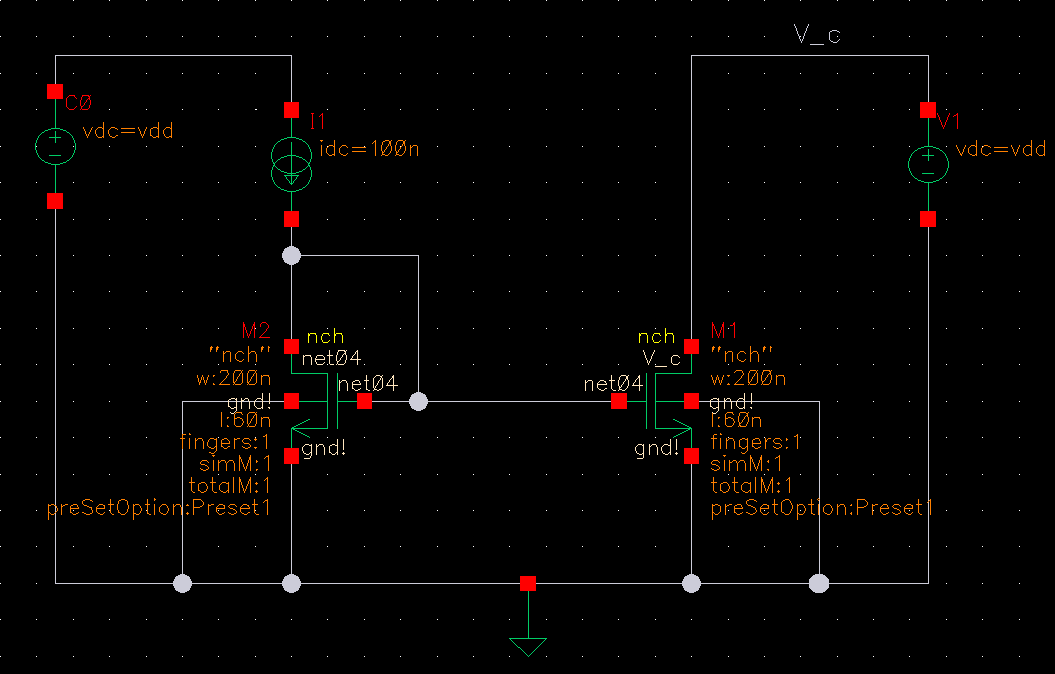
\includegraphics[width=0.8\textwidth]{circuit_c_fixed.png}
    \caption{Screencapture of the circuit in figure 1 c) from the lab manual simulated in Cadence.}
    \label{fig:circuitc}
\end{figure}

The bias current is implementet as a current mirror, consisting of $M2$ and $I4$, which sets the current that flows through $M1$.

\clearpage 

As suggested in the lab manual, a DC analysis is performed with $V_C$ as a sweep parameter. This results in the following plot:

\begin{figure}[h!]
    \centering
    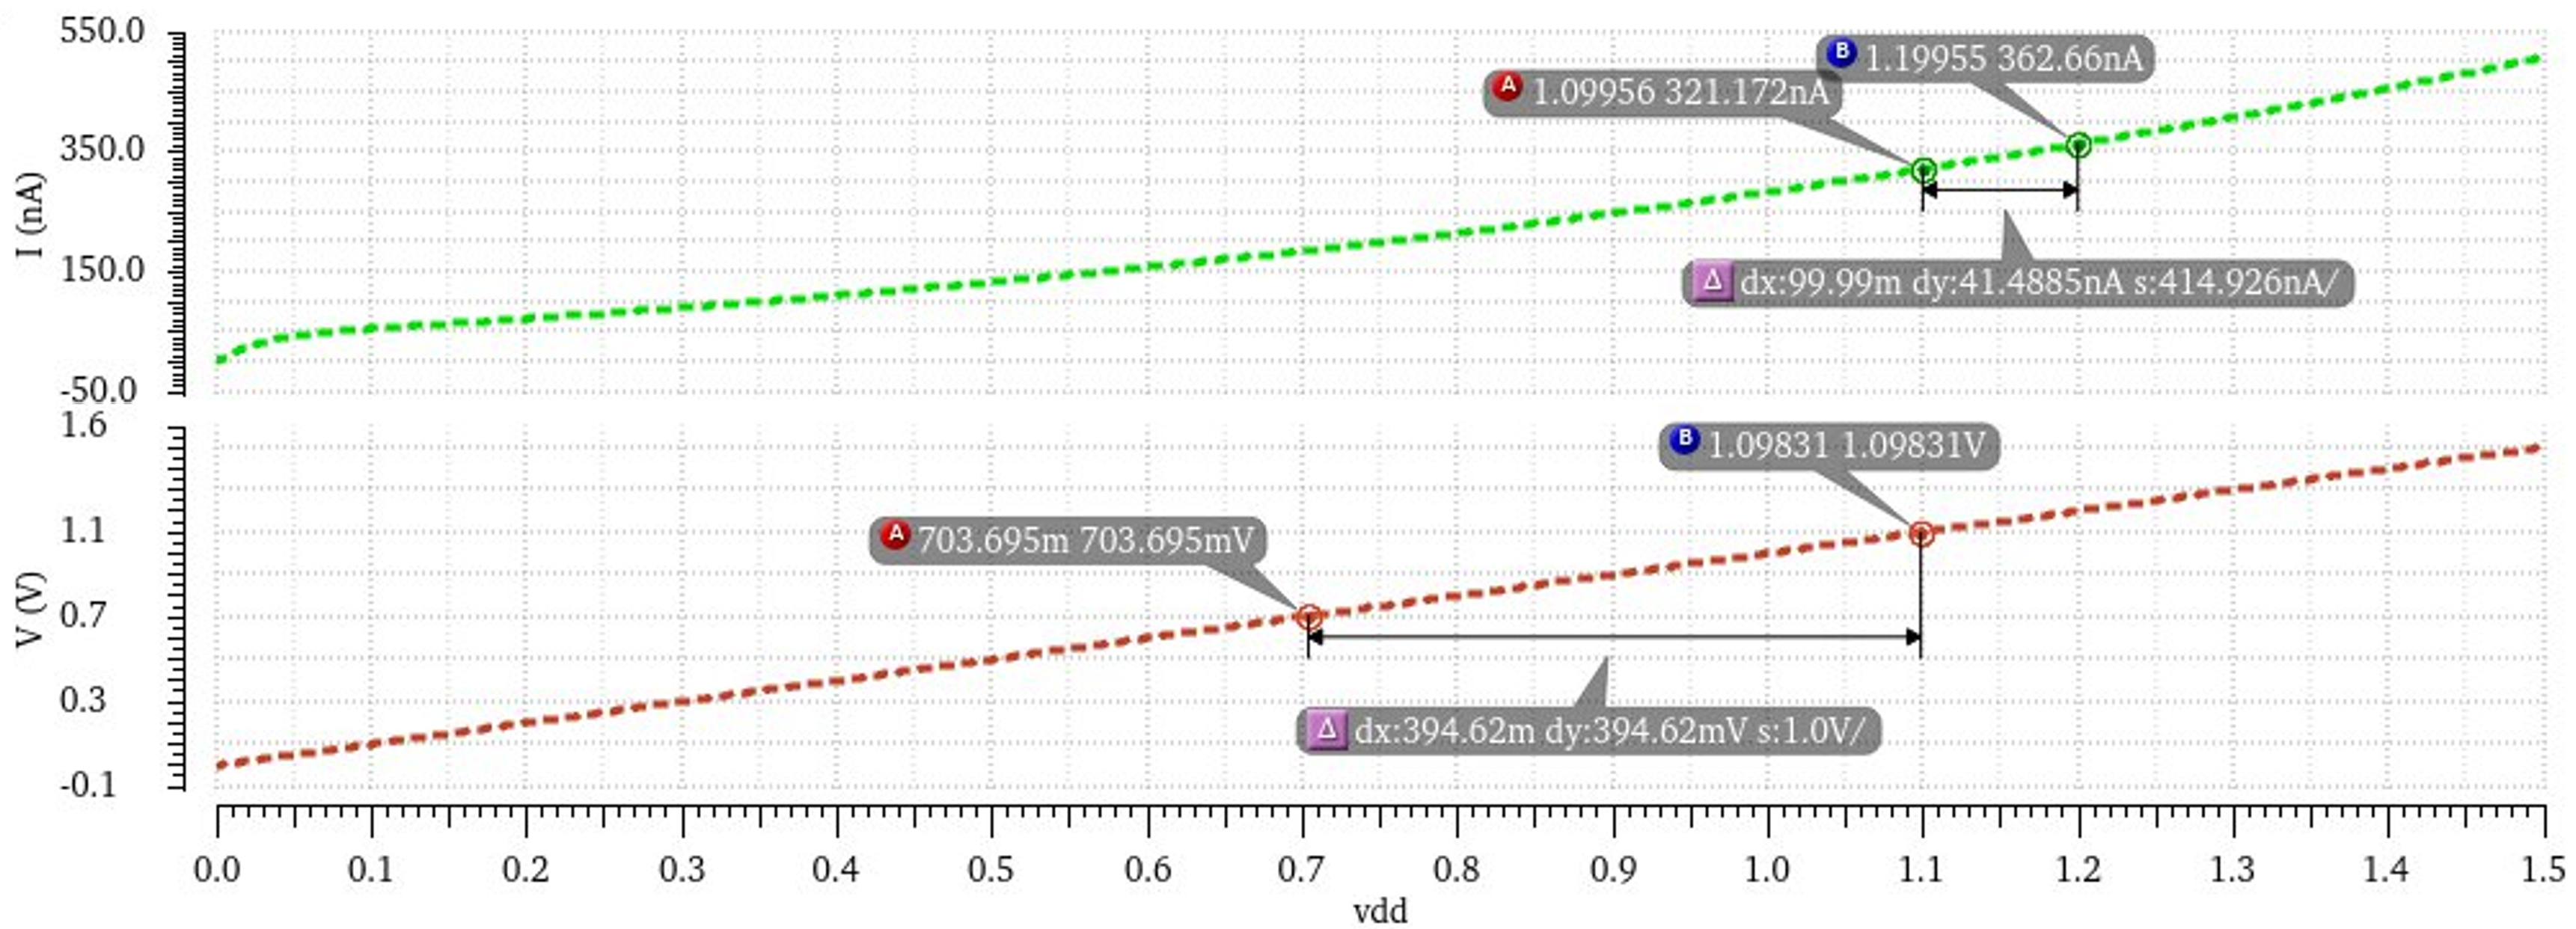
\includegraphics[width=0.8\textwidth]{plot_circuit_c_FINAL.png}
    \caption{Screencapture of the DC sweep of the circuit in figure 1.}
    \label{fig:plotc}
\end{figure}

$\Delta I_D$ is calculated as the difference between two points on the \textit{most linear} part of the curve. In figure \ref{fig:plotc}, this is chosen to be a segment at the end of the curve. The DC sweep simulation is set to sweep from $0 \ \text{V}$ to $1.5 \ \text{V}$, as the lab manual specifies to use only up to $1.2 \ \text{V}$, the last point is chosen to be close to $1.2 \ \text{V}$.
\begin{align}
    \Delta I_D &= 414.926 \ \text{nA}
\end{align}

The same method is used to calculate $\Delta V_{DS}$, however as $V_C$ is the sweep parameter, the voltage rises lineary. The difference between two points on this line will be the same wherever. In figure \ref{fig:plotc}, the points are chosen arbitrarily.

\begin{align}
    \Delta V_{DS} = 1 \ \text{V}
\end{align}
$R_{ds}$ can then simply be calculated using Ohms Law:
\begin{align}
    r_{ds} = \frac{\Delta V_{DS}}{\Delta  I_D} = \frac{ 1 \ \text{V}}{414.926 \ \text{nA}} = 2.4007 \ \text{M}\Omega
\end{align}

The next step is to change $\frac{W}{L}$ of $M0 \ (M1)$  in order to better it as a current source. For this rapport, the length was increased to $1 \  \mu m$ 
\begin{figure}[h!]
    \centering
    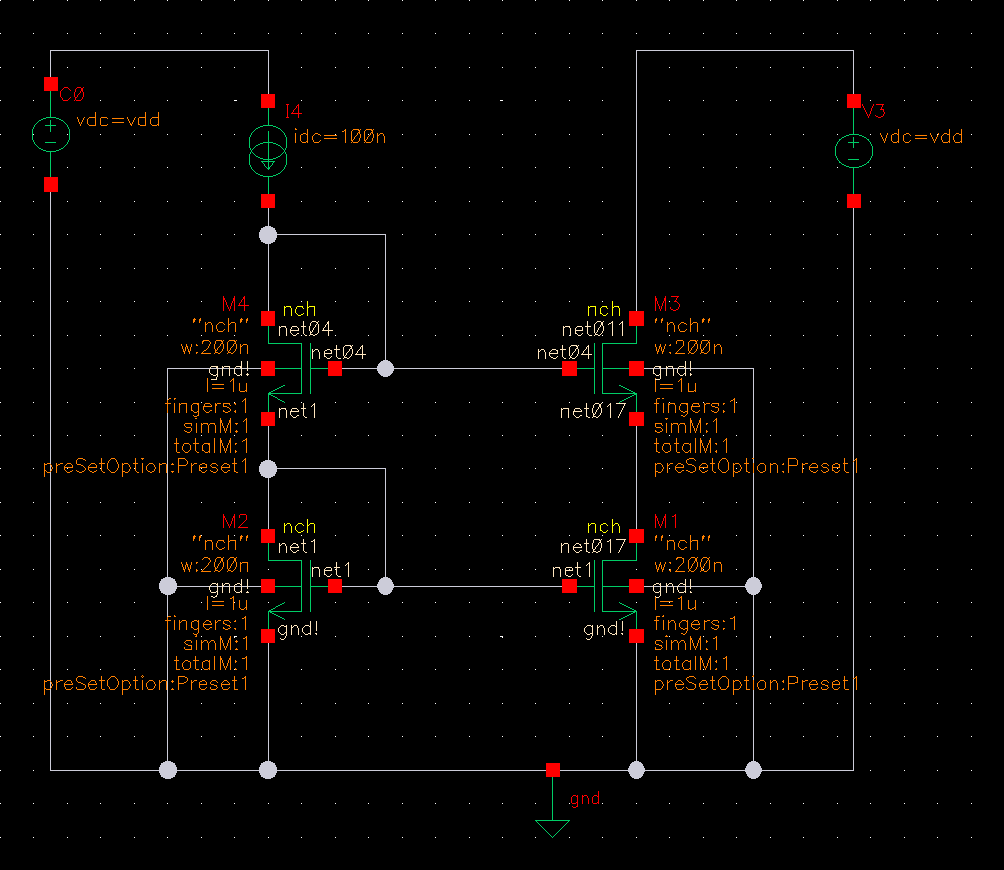
\includegraphics[width=0.8\textwidth]{circuit_d_cascode.png}
    \caption{Screencapture of the circuit in figure 1 d) from the lab manual simulated in Cadence.}
    \label{fig:circuitd}
\end{figure}

\begin{figure}[h!]
    \centering
    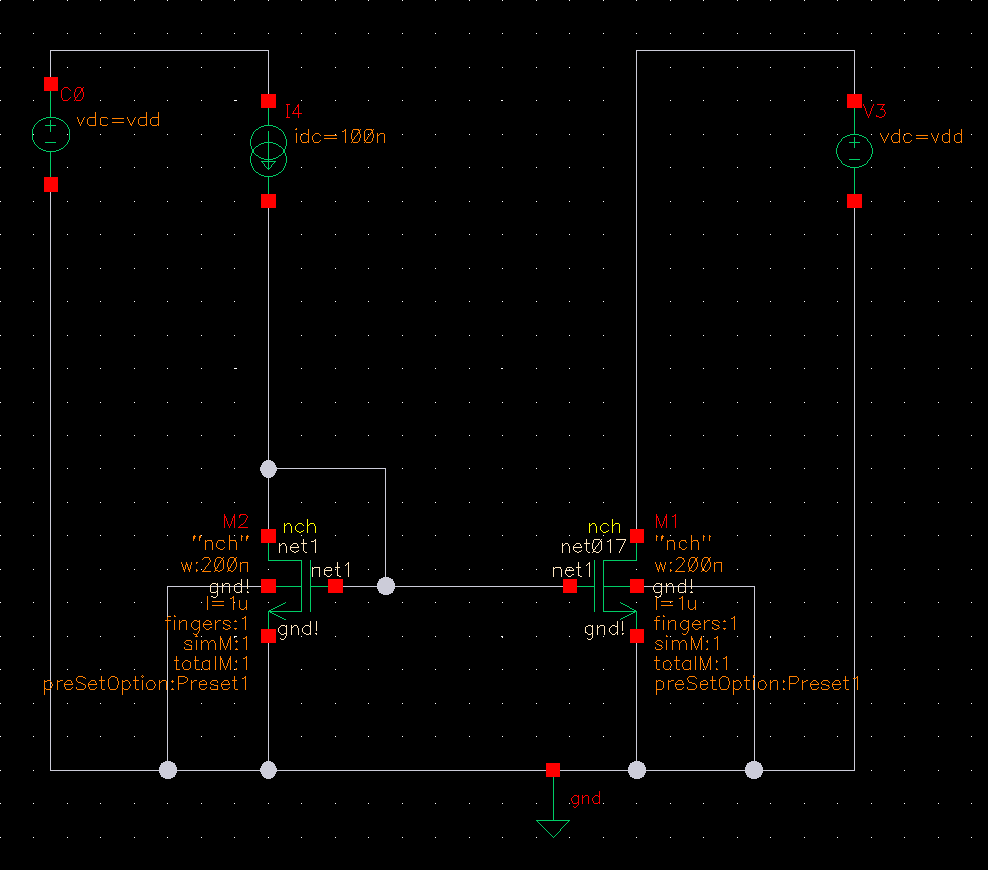
\includegraphics[width=0.8\textwidth]{circuit_d_simple.png}
    \caption{Screencapture of the circuit in figure 1 d) from the lab manual simulated in Cadence.}
    \label{fig:circuitdsimple}
\end{figure}

\begin{figure}[h!]
    \centering
    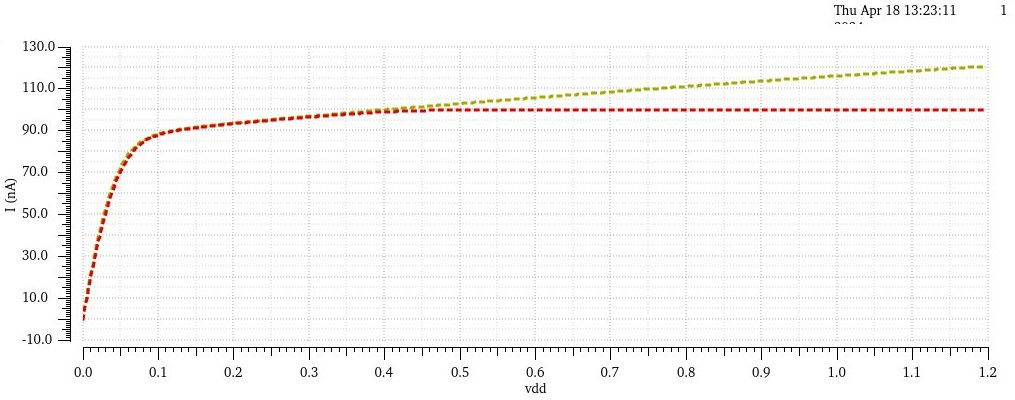
\includegraphics[width=1\textwidth]{plot_circuit_d_dc_sweep_omskjert.jpg}
    \caption{Screencapture of the DC sweep of both circuits in figure 1 d).}
    \label{fig:plotd}
\end{figure}


\end{document}